\section{Durchführung}
\label{sec:Durchführung}

\subsection{Aufbau}

Der Aufbau des Versuchs ist in Abbildung \ref{fig:aufbau} dargestellt. 

\begin{figure}[H]
    \centering
    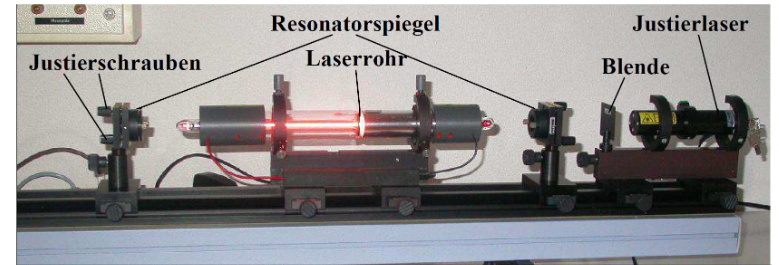
\includegraphics[scale=0.5]{content/aufbau.png}
    \caption{Darstellung des Aufbaus. \cite{alt}}
    \label{fig:aufbau}
\end{figure}

Die Justage wird mit Hilfe eines vorinstallierten Justierlasers ($\lambda = \SI{532}{\nano\metre}$, 
$P_\text{max} = \SI{1}{\milli\watt}$, $P_\text{grün} = \SI{0.2}{\milli\watt}$) durchgeführt. Die Maße des Laserrohrs liegen dabei 
für die Länge bei $l = \SI{408}{\nano\metre}$ und für den Durchmesser bei $\SI{1.1}{\milli\metre}$. Dieses ist mit dem HeNe-Gasgemisch 
im Verhältnis 5:1 gefüllt und mit Elektroden versehen, sodass mittels Entladung die Besetzungsinversion stattfinden kann. An den 
Enden des Laserrohrs befindet sich jeweils ein Brewster-Fenster, das dafür sorgt, dass eine definierte Polarisationsrichtung mit 
möglichst wenig Verlusten erreicht wird. Das Prinzip des Brewster-Fensters ist in Abbildung \ref{fig:brewster} zu sehen. 

\begin{figure}[H]
    \centering
    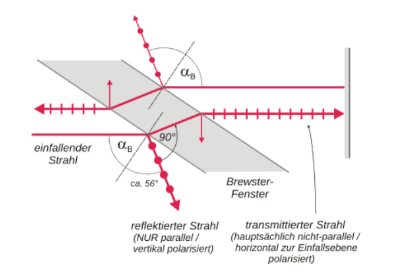
\includegraphics[scale=0.5]{content/brewster.png}
    \caption{Strahlengang am Brewster-Fenster. \cite{Zeugs}}
    \label{fig:brewster}
\end{figure}

Für den Resonator stehen konkave oder planparallele Spiegel zur Verfügung. 

\subsection{Durchführung}

Zunächst muss der Aufbau justiert werden. Dazu werden Laserrohr und Resonatorspiegel auf die Band gestellt und mittels des grünen
Justierlasers so ausgerichtet, dass die Rückreflexe der beiden Spiegel jeweils auf das Fadenkreuz der Justierblende treffen. 
Anschließend wird der Justierlaser abgestellt und die Hochspannung auf $\SI{6.5}{\milli\ampere}$ gestellt. 
Falls nicht direkt eine Lasertätigkeit einsetzt, muss vorsichtig an den Justierschrauben der Resonatorspiegel nachjustiert werden.

\subsubsection{Untersuchen der Stabilitätsbedingung}

Um die Stabilitätsbedingung zu untersuchen wird die Resonatorlänge in ungefähr $\SI{4}{\centi\metre}$ erhöht und jeweils die
Intensität mittels einer Photodiode gemessen. Dabei muss der Laser gegebenenfalls nach jeder Verschiebung der Spiegel nachjustiert
werden. Diese Messung wird für einen Resonator mit konkaven Spiegeln und einem Resonator mit einem konkaven und einem planparallelen
Spiegel durchgeführt.

\subsubsection{Multimodenbetrieb untersuchen}

Um den Multimodenbetrieb zu untersuchen, werden die Schwebefrequenzen vermessen. Dabei wird die Frequenz mittels einer schnellen 
Photodiode (Bandbreite bis $\SI{1}{\giga\hertz}$) gemessen und mittels eines Spektrumanalysators die Fourierspektren für 
unterschiedliche Resonatorlängen untersucht. 

\subsubsection{Bestimmung der Wellenlänge}

Zur Bestimmung der Wellenlänge werden unterschiedliche Gitter in den Strahlengang gestellt und der Abstand zwischen den Beugungsmaxima
mittels eines Zollstocks vermessen. 

\subsubsection{Bestimmung der Polarisation}

Um die Polarisation zu bestimmen, wird ein Polarisator hinter den Auskoppelspiegel gestellt. Die Polarisationsrichtung wird dann 
in $\SI{10}{\degree}$ geändert und jeweils die Intensität mittels einer Photodiode gemessen. 

\subsubsection{Untersuchen der $TEM$-Moden}

Zur Unterdrückung der Grundmode wird ein Wolframdraht der Dicke $d = \SI{0.005}{\milli\metre}$ zwischen Laserrohr und Resonatorspiegel
gebracht. Der Laserstrahl wird dann mittels einer Zerstreulinse aufgeweitet, sodass auf dem optischen Schirm dann verschiedene Moden
zu erkennen sein sollten. Die Intensität wird mittels einer Photodiode gemessen. 